% !TeX encoding = UTF-8
% 2023.12.06

\chapter{数学准备知识}\label{chtop}
%拓扑学是微分流形的先修课,本章简要介绍点集拓扑的初步知识.



\section{数个代数概念}
这小节只罗列一些后面章节会用到的代数概念,详尽内容请参考相应书籍.
列出这些概念的目的是为了便于查阅,以免再去频繁翻看其它书籍.

\begin{definition}\label{chtop:def_map}
    设有两个集合$M$和$N$,从$M$到$N$的{\heiti 映射}$\sigma$是指一个法则,
    它使$M$中每一个元素$a$都在$N$中存在{\uwave{唯一确定}}的元素$b$与之对应,
    记为$\sigma(a)=b$.$M$称为$\sigma$的{\heiti 定义域},
    $N$称为$\sigma$的{\heiti 陪域},
    集合$\sigma(M) \subset N$称为$\sigma$的{\heiti 值域}.
    
    元素$b$称为$a$在映射$\sigma$下的{\heiti 像};而
    $a$称为$b$在映射$\sigma$下的{\heiti 原像}.
    
    若$\forall a_1,a_2 \in M$都有$\sigma(a_1) \neq \sigma(a_2)$,则称
    映射$\sigma$是单一的,或{\heiti 单射}.
    
    若$\forall b\in N$在$M$中都至少存在一个原像$a$,
    则称映射$\sigma$是满的,或{\heiti 满射}.
    
    既单一又满的映射$\sigma$称为{\heiti 双射}或{\heiti 一一映射}.
    双射的逆是存在的,记为$\sigma^{-1}$.
\end{definition}


%由于多个概念都会用到数域,所以先介绍这个定义.
\begin{definition}\label{chtop:def_number-field}
    设$\mathbb{F}$是由一些复数组成的集合,其中包括$0$与$1$,
    如果$\mathbb{F}$中任意两个数(可以是相同的两个数)的
    和、差、积、商(除数不为0)仍是$\mathbb{F}$中的
    数(即对上述运算有封闭性),
    则称$\mathbb{F}$为一个{\heiti 数域}.\index[physwords]{数域}
\end{definition}
由$1+1=2,2+1=3,\cdots$可知自然数是$\mathbb{F}$中的元素;
再由$0-1=-1,0-2=-2,\cdots$全体整数也属于此集合;
还可继续作除法运算,任意两个整数的商也属于$\mathbb{F}$,
故全体有理数都是$\mathbb{F}$的元素;
所有有理数的和、差、积、商仍是有理数,
可见有理数集合$\mathbb{Q}$是一个数域.
任何其它数域必包含有理数域作为其子集.

本书只会涉及:实数域和复数域,即要么$\mathbb{F}=\mathbb{R}$,要么$\mathbb{F}=\mathbb{C}$.

%\subsection{群论简介}\label{chtop:sec_group}


\begin{definition}\label{chtop:def_group}
    设$G$是一个非空集合,定义$G$上的一个二元运算“$*$”,称为{\heiti 群乘法},
    从集合$G$中任意两个元素$a$和$b$(两者可相等)得
    到的$a*b$恒在$G$中(即群乘法是{\heiti 封闭的}).
    再给出关于群乘法的三条性质:
    
    \fbox{甲} 结合律:即$\forall a,b,c \in G$,恒有$(a*b)*c=a*(b*c)$;
    
    \fbox{乙} 单位元(也称为幺元):存在幺元$e\in G$使得$\forall a \in G$有$a*e=e*a=a$;
    
    \fbox{丙} 逆元:$\forall a \in G$,都存在元素$b\in G$使得$a*b=b*a=e$;记$a^{-1}=b$.
    
    如果集合$G$和群乘法只满足性质\fbox{甲},那么称$G$为{\heiti 半群}.
    如果集合$G$和群乘法只满足性质\fbox{甲}和\fbox{乙},那么称$G$为{\heiti 幺半群}.
    如果集合$G$和群乘法满足性质\fbox{甲}、\fbox{乙}和\fbox{丙},那么称$G$为{\heiti 群}.
    通常情况下会省略群乘号“$*$”.  %,即记成$a*b\equiv ab$
    \index[physwords]{群}\index[physwords]{群!半群}\index[physwords]{群!幺半群}
\end{definition}
群元素的数目称为群的{\heiti 阶},记为$g$.若$g$是有限的,则称为{\heiti 有限群};
否则称为{\heiti 无限群}.一般说来两个群元的乘积是不可交换的,即$ab\neq ba$;
如果对于任意两个群元都可以交换,称此群为{\heiti \bfseries Abel 群}或{\heiti 交换群}.

\begin{example}
    设集合只有一个元素$G=\{e\}$,规定群乘法为$e*e=e$,显然这符合群定义各条性质,
    这是最简单的群,只有一个单位元.称之为{\heiti 平凡群}.
\end{example}

\begin{example}
	$\mathbb{Z}_{2}\equiv \{+1,-1\}$,规定群乘法为整数乘法.  \index[physwords]{Z${}_2$}
\end{example}

\begin{example}
	全体整数对加法构成群,记为$(\mathbb{Z},+)$.注:整数集不是数域. 
\end{example}


\begin{example}
    将集合$G$取为数域$\mathbb{F}$,规定群乘法为此数域的加法,则$(\mathbb{F},+)$符合群定义各条性质,
    称之为数域$\mathbb{F}$的{\heiti 加法群};比如$(\mathbb{R},+)$等等.
\end{example}


\begin{example}
    将集合$G$取为扣除零元素之后集合$\mathbb{F}^*=\mathbb{F}\backslash \{0\}$,规定群乘法为此数域的数的乘法,
    则$(\mathbb{F}^*,\times)$符合群定义各条性质,称之为$\mathbb{F}^*$的{\heiti 乘法群}.
\end{example}

    \index[physwords]{群!子群}
    
\begin{definition}
    设$H$是群$G$的非空子集;在与$G$相同的群乘法下,
    如果集合$H$构成群(满足群的定义\ref{chtop:def_group});
    则称$H$为$G$的{\heiti 子群}.
\end{definition}

\begin{definition}
    设$H$为$G$的{子群},由固定的$g\in G$且$g\notin H$可生成
    子群$H$的{\heiti 左陪集}:$g H = \{g h \mid \forall  h \in H \}$;
    同样可生成子群$H$的{\heiti 右陪集}:$ Hg = \{ h g  \mid \forall  h \in H \}$.
\end{definition}

\begin{definition}\label{chtop:def_normal-subgroup}
    设$H$为$G$的子群,若对于任意$g\in G$都有$g h g^{-1} \in H, \ \forall h\in H$;
    则称$H$为$G$的{\heiti 正规子群}或{\heiti 不变子群}.
\end{definition}
    
    \index[physwords]{群!不变子群}\index[physwords]{群!正规子群}
    
\begin{definition}\label{chtop:def_tttg}
    若从群$G$到群$F$存在一个映射$\phi:G\to F$保持群乘法不变,
    即$\forall g,h\in G$都有$\phi(gh)=\phi(g)\phi(h)$;
    则称映射$\phi$为群$G$到群$F$的{\heiti 同态映射};
    若$\phi$是满射,则称为{\heiti 满同态};若$\phi$是单射,则称为{\heiti 单同态};
    若$\phi$为双射,则称之为{\heiti 同构映射},记为$G \cong F$.
\end{definition}
    \index[physwords]{同态映射}\index[physwords]{同构映射}
    
\begin{definition}\label{chtop:def_kernel}
    若$\phi$是$G$到$F$的同态映射,$F$单位元$e$的原像集
    合${\rm ker}\phi = \phi^{-1}(e)=\{x\in G \ |\ \phi(x)=e\}$称
    为$\phi$的{\heiti 同态核},简称{\heiti 核} .
\end{definition}

    \index[physwords]{核} \index[physwords]{同态核|see{核}}

\begin{definition}\label{chtop:def_center}
    群$G$的{\heiti 中心}定义为:$C(G)=\{x\in G\ |\ xy=yx, \forall y\in G\}$.
\end{definition}

如果群$G$有不变子群$H$,则可以证明(\parencite[\S 1.3]{mengdj-cxds-1})商集$G/H$也是群,
称为群$G$对$H$的{\heiti 商群}.商群$G/H$中的元素是$G$中$H$的所有陪集,单位元是$H$.
存在从$G$到$G/H$的映射$\boxed{\pi (g)= gH,\ \forall g\in G}$,
则$\pi$是同态映射,称为{\heiti 自然同态}.
我们不加证明地引入群同态基本定理(证明过程可参考\parencite[\S 1.7]{mengdj-cxds-1}或类似书籍):

\begin{theorem}\label{chtop:thm_ghk}
    $f$是群$G$到群$K$的同态映射,则有如下结论:
    {\bfseries (1)} ${\rm ker}f$是群$G$的不变子群.
    {\bfseries (2)} 设$\pi$是从$G$到商群$G/{\rm ker}f$的自然同态,
    则有从$G/{\rm ker}f$到$K$上的同构映射$\bar{f}$使得$f=\bar{f}\circ \pi$.
    {\bfseries (3)} 若另有$G$的不变子群$N$,并且${\rm ker}f\subset N$,
    则$G/N \cong K/f(N)$(同构).
    {\bfseries (4)}  继(3)中记号;$\pi'$是从$G$到$G/N$的自然同构,
    另有$G$的不变子群$H$,并且$H\subset N$;
    则将(3)中的$K$换成$G/H$,$f$换成$\pi'$,有$G/N \cong (G/H)/(N/H)$(同构).
\end{theorem}

    \index[physwords]{一般线性群GL}
    
\begin{example}
    全体可逆、$\mathbb{F}$数值、$n$维矩阵构成一个集合,并取矩阵的乘法为群乘法,
    则此集合构成一个群,称为$\mathbb{F}$值{\heiti 一般线性群}(General Linear group),
    记为$GL(n,\mathbb{F})$.比如实一般线性群$GL(n,\mathbb{R})$,复一般线性群$GL(n,\mathbb{C})$.
\end{example}

\begin{example}
    给定$\mathbb{F}$上的线性空间$V$,空间$V$上全体可逆线性变换构成一个集合,
    取群乘法为两个线性变换相继作用,则此集合构成群,也称为{\heiti 一般线性群},记作$GL(n,V)$.
    因为选定基底后,可逆线性变换与可逆矩阵有双射关系,所以$GL(n,\mathbb{F})$同构于$GL(n,V)$.
\end{example}


\begin{definition}\label{chtop:def_group_representation}
    如果存在从群$G$到一般线性群$GL(n,V)$的同态映射$\phi:G\to GL(V)$,
    则称$(\phi,V)$为群$G$的一个$n$维{\heiti 线性表示},
    简称{\heiti 表示}. 如果$\phi$是同构映射,则成为{\heiti  忠实表示}.
    非空的$V$是表示空间,其维数称为表示的{\heiti 维数}.
\end{definition}
    \index[physwords]{群!群表示}
    
\begin{definition}
    群$G$的线性表示$(\phi,V)$的子空间$V_1$若满足$\phi(g)V_1 = V_1,\forall g\in G$,
    则$V_1$称为$G$的{\heiti 不变子空间};
    于是$(\phi|_{V_1},V_1)$可称为表示$(\phi,V)$的{\heiti 子表示}.
\end{definition}

\begin{definition}\label{chtop:def_irreducible-representation}
    若除$\{0\}$和$V$外,$G$的表示$(\phi,V)$没有不变子空间,则称$\phi$是{\heiti 不可约表示}.
    否则称为{\heiti 可约表示}.若对任意不变子空间$V_1$(除$\{0\}$和$V$外),
    存在不变子空间$V_2$使得$V=V_1\oplus V_2$(直和),则称$G$的表示$(\phi,V)$是{\heiti 完全可约的};
    此时记$\phi=\phi|_{V_1}\oplus \phi|_{V_2}$,称$\phi$是子表示$\phi|_{V_1}$与$\phi|_{V_2}$的{\heiti 直和}.
\end{definition}


\begin{definition}
    设$(\phi,V)$和$(\psi,U)$是群$G$的两个表示;若存在\uwave{线性同构}映
    射$\mathcal{A}:V\to U$使得$\mathcal{A}\phi(g) = \psi(g)\mathcal{A},\, \forall g\in G$成立,
    则称表示$(\phi,V)$和$(\psi,U)${\heiti 等价}.
\end{definition}

%寻找群的不等价、不可约表示是表示论的核心课题.


\begin{definition}
    设$\Omega$是任一非空集合,$\Omega$到自身的所有{\kaishu 双射}组成的集合
    (记为$S(\Omega)$)对映射乘法构成一个群,称之为$\Omega$上的{\heiti 全变换群};
    $S(\Omega)$的任一子群称为$\Omega$上的{\heiti 变换群}.
    当$\Omega$是$n$个有限元素的集合时,$\Omega$到自身的{\kaishu 双射}称为
    一个{\heiti $\boldsymbol{n}$元置换};$S(\Omega)$上的全体变换
    称为{\heiti $\boldsymbol{n}$元对称群},记为$S_n$;
    $S_n$自身及子群也称为{\heiti 置换群}.
\end{definition}

\index[physwords]{群!变换群}    \index[physwords]{群!置换群}

\begin{example}\label{chtop:exm_ZhiHuanQun}
    本例给出置换群具体形式.
    设有$n$相同的抽屉,每个抽屉上贴有编号,从$1$到$n$;$1$号抽屉里面放着物体$A$,
    $2$号抽屉里面放着物体$B$,……,以此类推.
    现在我们将第$1$抽屉中的物体放到第$a_1$个抽屉,
    将第$2$抽屉中的物体放到第$a_2$个抽屉,……,
    将第$n$抽屉中的物体放到第$a_n$个抽屉.
    我们将这个操作记成:
    $(\begin{smallmatrix}
    	1 &2 &\cdots &n \\  a_1 &a_2 &\cdots &a_n
    \end{smallmatrix} )$
    其中$1, 2, \cdots, n$表示物体所在原来的抽屉,
    $a_1, a_2, \cdots, a_n $表示物体所在新的抽屉编号.
    这些操作的集合构成$n$阶{\kaishu 置换群}$S_n$.
    下面以三个客体$A,B,C$为例来说明这个操作该过程.
    \begin{equation*}
        \young(ABC) \xrightarrow{\left(\begin{smallmatrix}
                1 &2 &3 \\  2 & 3 & 1  \end{smallmatrix} \right)}
        \young(CAB) \xrightarrow{\left(\begin{smallmatrix}
                1 &2 &3 \\  2 & 3 & 1  \end{smallmatrix} \right)}
        \young(BCA) \xrightarrow{\left(\begin{smallmatrix}
                1 &2 &3 \\  2 & 3 & 1  \end{smallmatrix} \right)}
        \young(ABC)
    \end{equation*}
    设有两个置换$S=(\begin{smallmatrix}
    	1 &2 &\cdots &n \\  a_1 &a_2 &\cdots &a_n
    \end{smallmatrix} )$、$T=(\begin{smallmatrix}
    a_1 &a_2 &\cdots &a_n \\ b_1 &b_2 &\cdots &b_n 
    \end{smallmatrix} )$
    则两个置换的乘法定义为:
    \begin{equation*}
    	TS\equiv 
    	\begin{pmatrix} a_1 &a_2 &\cdots &a_n \\ b_1 &b_2 &\cdots &b_n \end{pmatrix}
    	\begin{pmatrix} 1 &2 &\cdots &n \\  a_1 &a_2 &\cdots &a_n \end{pmatrix}
    	=\begin{pmatrix} 1 &2 &\cdots &n \\  b_1 &b_2 &\cdots &b_n \end{pmatrix} .
    \end{equation*}
    即先实行置换操作$S$,再实施置换操作$T$.\qed
\end{example}

%\subsection{环体域模}
\begin{definition}\label{chtop:def_ring}
    设$R$是非空集合,在此集合上定义了两个代数运算(对运算有封闭性),一个叫做{\kaishu 加法},
    记作$a+b$,另一个叫做{\kaishu 乘法},记作$ab$;并且这两个运算满足如下六条规则:
    
    {\bfseries (1)} 加法结合律,即$(a+b)+c=a+(b+c)$;
    
    {\bfseries (2)} 加法交换律,即$a+b=b+a$;
    
    {\bfseries (3)} 在$R$中存在零元素$0$,使得$a+0=a$;
    
    {\bfseries (4)} 对$R$中元素$a$,存在$d\in R$使得$a+d=0$,$d$称为$a$的负元素;
    
    {\bfseries (5)} 乘法结合律,即$(ab)c=a(bc)$;
    
    {\bfseries (6)} 乘法对加法有左右分配律,即$a(b+c)=ab+ac,\ (b+c)a= ba + ca$.
    
    其中$a,b,c$是$R$中任意元素,则称$R$是一个{\heiti 环}(ring).
\end{definition}

环$R$对其加法构成交换群,对其乘法构成半群.

容易证明环$R$中的零元和负元是唯一的;利用负元可以定义减法.
如果环$R$中有一个元素$e$对乘法具有如下性质:
$e a = a e  =a, \ \forall a \in R $;
则称$e$是$R$中的{\heiti 幺元}或单位元,此时环$R$称为{\heiti 幺环}或者
有单位元的环;可证单位元是唯一的,通常会用“$1$”来代替$e$.

如果环$R$的乘法还有交换律,即$ab=ba$,则称其为{\heiti 交换环}.

在幺环$R$中,对于$a\in R$,如果存在$b\in R$,使得$ab=ba =1$,
则称$a$是可逆的,$b$称为$a$的逆元,逆元是唯一的,一般记为$a^{-1}$.

如果环$R$中有元素$b\neq 0$,存在元素$a\neq 0$使得$ab=0$(或$ba=0$),则称
元素$a$为$R$的一个{\heiti 左}(或{\heiti 右}){\heiti 零因子},两者
都可简称为{\heiti 零因子}.元素0也可称为(平凡)零因子.
任何两个非零元素之积不为零的环称为{\heiti 无零因子环}.

有单位元(且$1\neq 0$)的无零因子环称为{\heiti 整环}(domain);注意不是整数环.

\begin{example}
    一切数域都是环;且是有幺元的交换环.
\end{example}

\begin{example}
    整数集$\mathbb{Z}$对其自身的加法和乘法构成环,称为{\heiti 整数环}.
    此环不是数域.
\end{example}

如果环$R$的非零元素集合对乘法构成群(且$1\neq 0$),则称为{\heiti 体}.

可交换的体称为{\heiti 域},即环$R$中非零元素集合对乘法构成交换群.


环和域还有{\kaishu 特征}(Characteristic)概念;
此处想声明的是:所有\uwave{数域}特征为{\kaishu 零}.
(比如可参阅\parencite[\S 3.1]{mengdj-cxds-1}中叙述,或查阅类似文献)


设$f(x)$是非常值一元多项式,其系数属于域$\mathbb{F}$;若$f(x)$在$\mathbb{F}$中至少有一个根,
则域$\mathbb{F}$称为{\heiti 代数闭域}.容易验证复数域是代数闭的.
多项式$f(x)=x^2+1$在实数域没有根,故实数域不是代数闭的.

\index[physwords]{代数闭域}
\index[physwords]{四元数}

生于爱尔兰都柏林的数学家、力学家哈密顿(William Rowan Hamilton 1805~1865)
于1843年发明了{\heiti 四元数}(quaternion)如下  
\begin{equation}\label{chtop:eqn_quaternion}
    a+b \mathbbm{i} +c\mathbbm{j} +d \mathbbm{k}, \qquad \forall a,b,c,d \in \mathbb{R}.
\end{equation}
其中符号$\mathbbm{i,j,k}$满足,
\begin{equation*}
    \mathbbm{i}^2 = \mathbbm{j}^2 = \mathbbm{k}^2 = -1; \quad
    \mathbbm{i}\mathbbm{j}=-\mathbbm{j}\mathbbm{i}=\mathbbm{k}, \quad
    \mathbbm{j}\mathbbm{k}=-\mathbbm{k}\mathbbm{j}=\mathbbm{i}, \quad
    \mathbbm{k}\mathbbm{i}=-\mathbbm{i}\mathbbm{k}=\mathbbm{j}.
\end{equation*}
所有四元数组成的集合记为$\mathbb{H}$,规定$\mathbb{H}$的加法和乘法与复数类似,即
\begin{equation*}
    a+b \mathbbm{i} +c\mathbbm{j} +d \mathbbm{k}
    + a'+b' \mathbbm{i} +c'\mathbbm{j} +d' \mathbbm{k}
    \overset{def}{=} (a+a')+ (b+b')\mathbbm{i} +(c+c')\mathbbm{j} + (d+d') \mathbbm{k} .
\end{equation*}
和
\begin{align*}
    (a&+b \mathbbm{i} +c\mathbbm{j} +d \mathbbm{k} )
    (a'+b' \mathbbm{i} +c'\mathbbm{j} +d' \mathbbm{k})
    \overset{def}{=} aa'+ ab' \mathbbm{i} +ac'\mathbbm{j} +ad' \mathbbm{k}
    + ba'\mathbbm{i}+bb' \mathbbm{i}\mathbbm{i} \\
    &+bc'\mathbbm{i}\mathbbm{j} +bd' \mathbbm{i}\mathbbm{k}
    + ca'\mathbbm{j}+cb' \mathbbm{j}\mathbbm{i} +cc'\mathbbm{j}\mathbbm{j} +cd' \mathbbm{j}\mathbbm{k}
    + da'\mathbbm{k}+db' \mathbbm{k}\mathbbm{i} +dc'\mathbbm{k}\mathbbm{j} +dd' \mathbbm{k}\mathbbm{k} \\
    =&aa'-bb'-cc'-dd' + (ab'+ba'+cd'-dc')\mathbbm{i} \\
    &+ (ac'+ca'-bd'+db')\mathbbm{j} + (ad' +da' +bc'-cb')\mathbbm{k} .
\end{align*}
很明显四元数对于乘法不具有对易性.
容易验证全体四元数$\mathbb{H}$是{\kaishu 体},但不是{\kaishu 域}.
由此可见定义\ref{chtop:def_number-field}将取值范围限制在复数集合是合理的.

\begin{definition}\label{chtop:def_module}
    设$R$是一交换环,有一个非空的集合$M$,如它满足下列条件:    
    {\bfseries (1)} $M$中有加法“$+$”,而对“$+$”而言,$M$是一交换群;取此加法群的幺元为$0$.    
    {\bfseries (2)} $\forall a\in R,\ m\in M$,有二元运算(通常称为乘法“$*$”)存在,
    使$a*m\in M$,及$1*m=m$,其中“1”($1\neq 0$)是环$R$乘法的幺元(乘法符号“$*$”经常忽略不写).    
    {\bfseries (3)} 交换环$R$的加法、乘法,$M$的加法及$R$与$M$之间的乘法都适合结合律及分配律,
    即(其中任取$a,b\in R;\ m,n\in M$)
    \begin{equation*}
        (a b ) m = a (b m), \quad (a + b)m=a m+ b m, \quad
        a(m+n) = a m + a n.
    \end{equation*}
    则称$M$为$R$-{\heiti 模},或简称为{\heiti 模}.
\end{definition}

\begin{example}\label{chtop:exm_VM}
    数域$\mathbb{F}$上的线性空间$V$(见定义\ref{chmla:def_linear-space})可以看成$\mathbb{F}$-模.
\end{example}




%\subsection{非数域的域}\label{chtop:sec_NaNfield}
%是否存在非数域的域呢?为了描述这个问题,需要分成数个部分.
%
%在集合$A$中有一个二元运算“$\sim$”.有如下三个条件:
%{\bfseries (1)} {\kaishu 自反性},即$a\sim a$.
%{\bfseries (2)} {\kaishu 对称性},即若$a \sim b$,则$b\sim a$.
%{\bfseries (3)} {\kaishu 传递性},即若$a \sim b$且$b \sim c$,则$a\sim c$.
%其中$a,b,c$是$A$中任意元素.
%如果“$\sim$”满足上述三个条件,则称“$\sim$”是集合$A$中的{\heiti 等价关系}.
%
%\index[physwords]{等价关系}
%\index[physwords]{商集}  \index[physwords]{自然映射}
%
%设集合$A$中有等价关系“$\sim$”.$A$中所有关于“$\sim$”等价的元素构成的集合$\{K_a \}$,
%称为$A$对“$\sim$”的{\heiti 商集},记为$A/\sim$.
%由$\boxed{\pi(a) = K_a,\ \forall a\in A}$定义了一个从$A$到$A/\sim$映射,
%我们称$\pi$为{\heiti 自然映射}.显然$\pi$是满射,但一般情况下不是单一的.
%
%
%\begin{definition}
%    若环$R$的非空子集$S$对$R$的加法、乘法也构成环,则称$S$是$R$的{\heiti 子环}.
%    若$S$还满足$RS\subset S$(或$SR\subset S$),则称$S$是$R$的{\heiti 左理想}(或{\heiti 右理想}).
%    若$S$既是左理想又是右理想,则称之为{\heiti 双边理想},简称{\heiti 理想}.
%\end{definition}
%
%若$I$是环$R$的双边理想,则可在商集$R/\sim \equiv R/I$中定义加法、乘法如下:
%\begin{equation}
%    (a+I)+(b+I)\overset{def}{=} (a+b)+I,\quad
%    (a+I)\cdot (b+I)\overset{def}{=} (ab)+I;\quad \forall a,b \in R.
%\end{equation}
%可以证明(\parencite[\S 1.4]{mengdj-cxds-1}):商集$R/I$对上述加法、乘法也构成环,
%称为$R$对$I$的{\heiti 商环}.
%
%\begin{definition}
%    设有两个环$R$、$S$.$\varphi$是从$R$到$S$的映射,如果
%    \begin{equation}
%        \varphi (a+b) = \varphi(a) + \varphi(b),\quad
%        \varphi (a\cdot b) = \varphi(a) \cdot \varphi(b); \quad \forall a,b \in R
%    \end{equation}
%    成立,则称$\varphi$是从$R$到$S$的{\heiti 同态}.
%    若$\varphi$是满射,则称之为{\heiti 满同态}.
%    若$\varphi$是双射,则称之为{\heiti 同构},记为$R \cong S$.
%\end{definition}
%
%$R$到其商环$R/I$的映射$\boxed{\pi (x) = x+ I \, (\forall x\in R)}$是
%同态映射,称$\pi$为{\heiti 自然映射}.
%
%\begin{theorem}\label{chtop:thm_rhk}
%    (环同态基本定理)$f$是环$R$到环$R'$的同态映射,则有如下结论:
%    {\bfseries (1)} ${\rm ker}f$是环$R$的双边理想.
%    {\bfseries (2)} 设$\pi$是从$R$到商环$R/{\rm ker}f$的自然同态,
%    则有$R/{\rm ker}f$到$R'$上的同构映射$\bar{f}$使得$f=\bar{f}\circ \pi$.
%    {\bfseries (3)} 若另有$R$的双边理想$I$,并且${\rm ker}f\subset I$,
%    则$R/I \cong R'/f(I)$(同构).
%    {\bfseries (4)}  继(3)中记号;$\pi'$是从$R$到$R/I$的自然同构,
%    另有$R$的双边理想$A$,并且$A \subset I$;则
%    将(3)中的$R'$换成$R/A$,$f$换成$\pi'$,有$R/I \cong (R/A)/(I/A)$.
%\end{theorem}
%定理\ref{chtop:thm_rhk}证明过程可参考\parencite[\S 1.7]{mengdj-cxds-1}或类似书籍.
%
%
%设正整数$p\in \mathbb{Z}$,令$\boxed{p\mathbb{Z}\equiv \{p a\mid a \in \mathbb{Z} \}}$,
%则$p\mathbb{Z}$是整数加法群$(\mathbb{Z},+)$的子群,且是不变子群.
%则可定义商群$\boxed{\mathbb{Z}_p \equiv \mathbb{Z}/p\mathbb{Z}}$.
%
%举个具体的例子,令$p=3$,则有$3\mathbb{Z}=\{\cdots,-6,-3,0,3,6,\cdots \}$.
%$3\mathbb{Z}$还有两个陪集$p_1=\{\cdots,-5,-2,1,4,7,\cdots \}$、
%$p_2=\{\cdots,-4,-1,2,5,8,\cdots \}$.
%根据同态核定理商群$\mathbb{Z}_3$有三个元素$\{3\mathbb{Z},p_1,p_2\}$,
%我们一般把它记成$\mathbb{Z}_3=\{\bar{0},\bar{1},\bar{2}\}$.
%推而广之$\boxed{\mathbb{Z}_p=\{\bar{0},\bar{1},\cdots,\overline{p-1}\}}$.
%
%
%\index[physwords]{同余}
%下面给商群$\mathbb{Z}_p$再赋予“加法”和“乘法”,使之成为环.为此先介绍同余的概念.
%
%整数环$\mathbb{Z}$中有元素$a,b,p$,其中$p\neq 0$;数$a$、$b${\heiti 同余}是指:
%\begin{equation}
%    \frac{a}{p}\text{和} \frac{b}{p} \text{的余数相同,记为}\ 
%    a\equiv b ({\rm mod} p).
%\end{equation}
%
%容易验证同余是一种等价关系,将其记为$a \sim b$.
%
%不难发现$3\mathbb{Z}$及其陪集$p_1$、$p_2$内的整数都是同余关系;
%$3\mathbb{Z}$中的数除以$3$余数是$0$,$p_1$中的数除以$3$余数是$1$,$p_2$中的数除以$3$余数是$2$.
%这种同余关系属性同样适用于$\mathbb{Z}_p$,这也是我们将其中元素记为$\bar{0},\bar{1},\cdots,\overline{p-1}$的原因.
%$\forall \bar{a},\bar{b},\bar{c}\in \mathbb{Z}_p$,不难验证同余关系满足
%\begin{equation}\label{chtop:eqn_Zppt}
%    \overline{a+b}=\bar{a}+\bar{b},\qquad \overline{a \cdot b}=\bar{a}\cdot \bar{b} .
%\end{equation}
%上式中加法和乘法就是整数的加法和乘法.
%我们把上式中的加法和乘法当成$\mathbb{Z}_p$中的“加法”、“乘法”定义,
%这样$\mathbb{Z}_p$中便有了“加法”和“乘法”.
%容易证明$\mathbb{Z}_p$对于“加法”构成对易群.
%两个整数相除可能不再是整数,故上述定义的“乘法”没有逆,也就是此“乘法”不构成群,
%但可以证明构成幺半群.这两个证明都不困难,留给读者当练习.
%故有:$\mathbb{Z}_p$对于式\eqref{chtop:eqn_Zppt}中定义的“加法”构成Abel群,对于“乘法”构成幺半群.
%
%式\eqref{chtop:eqn_Zppt}的“加法”和“乘法”还具有分配律(反复利用式\eqref{chtop:eqn_Zppt}中的关系):
%\begin{equation}
%    \bar{a}(\bar{b}+\bar{c}) = \bar{a}(\overline{b+c})=\overline{a(b+c)}
%    =\overline{ab+ac}= \bar{a}\bar{b}+\bar{a}\bar{c} .
%\end{equation}
%从上式可知$\mathbb{Z}_p$满足可对易幺环的定义.
%
%$\mathbb{Z}_p$中的零元是$\bar{0}$,扣除零元后,我们考察剩余元素对“乘法”是否构成群.
%一般而言,仍旧不是群(对乘法的逆运算——除法——不封闭).
%若我们要求\uwave{\kaishu $p$是正素数},那么对于任意的正整数$a<p$,存在整数$m$、$n$使得
%如下关系:$m a + n p =1$成立;进而有
%\begin{equation}
%    \bar{1}=\bar{m}\bar{a}+\bar{n}\bar{p}=\bar{m}\bar{a}+\bar{n}\bar{0}=\bar{m}\bar{a}
%    \quad \Rightarrow \quad \bar{m}\bar{a} = \bar{1} .
%\end{equation}
%这样便证明了:当$p$是素数时,$\mathbb{Z}_p$中非零元素都可逆,进而全体非零元素构成群.
%故,只含$p$个元素的可对易幺环$\mathbb{Z}_p$($p$是素数)是{\kaishu 域},但不是数域.


\begin{exercise}
	请验证四元数是体.
\end{exercise}

\section{点集拓扑基本概念}\label{chtop:sec_topology}
我们先给出点集拓扑的一些概念(都取自\parencite{munkres-2000-topology}相应章节),
这些概念大都晦涩难懂;
之后我们把这些概念应用到度量空间上(如$\mathbb{R}^m$),以便更好的理解.

\begin{definition}\label{chtop:def_top}
    非空集合$X$上的一子集族$\mathscr{T}$,它满足如下条件:
    {\bfseries (1)} $X$和$\varnothing$都在$\mathscr{T}$中;
    {\bfseries (2)} $\mathscr{T}$的任意子族元素的并在$\mathscr{T}$中;
    {\bfseries (3)} $\mathscr{T}$任意两个子族元素的交在$\mathscr{T}$中.
    则称集合$X$指定了一个{\heiti 拓扑}$\mathscr{T}$;
    称$X$为{\heiti 拓扑空间},记为$(X,\mathscr{T})$,可简记为$X$;
    $\mathscr{T}$中元素称为{\heiti 开集}.
    \index[physwords]{拓扑} \index[physwords]{拓扑空间} \index[physwords]{开集}
\end{definition}

只要满足上面定义中的三条公理就可以称为拓扑.

\begin{example}
    设$X$是由三个元素$\{a,b,c\}$组成的集合,其上有很多拓扑;参见图\ref{chtop:pic_top}.
\end{example}

    
左上$\mathscr{T}_1$:开集有$X$、$\varnothing$.

左中$\mathscr{T}_2$:开集有$X$、$\varnothing$、$\{b\}$.

左下$\mathscr{T}_3$:开集有$X$、$\varnothing$、$\{a, b\}$.

中上$\mathscr{T}_4$:开集有$X$、$\varnothing$、$\{a\}$、$\{a,b\}$.

中中$\mathscr{T}_5$:开集有$X$、$\varnothing$、$\{a\}$、$\{b,c\}$.

中下$\mathscr{T}_6$:开集有$X$、$\varnothing$、$\{a\}$、$\{b\}$、$\{a, b\}$.

右上$\mathscr{T}_7$:开集有$X$、$\varnothing$、$\{b\}$、$\{a,b\}$、$\{b,c\}$.

右中$\mathscr{T}_8$:开集有$X$、$\varnothing$、$\{b\}$、$\{c\}$、$\{a,b\}$、$\{b,c\}$.

右下$\mathscr{T}_9$:开集有$X$、$\varnothing$、$\{a\}$、$\{b\}$、$\{c\}$、$\{a, b\}$、$\{a, c\}$、$\{ b,c\}$.
\qed


\begin{figure}[htb]
    \centering
    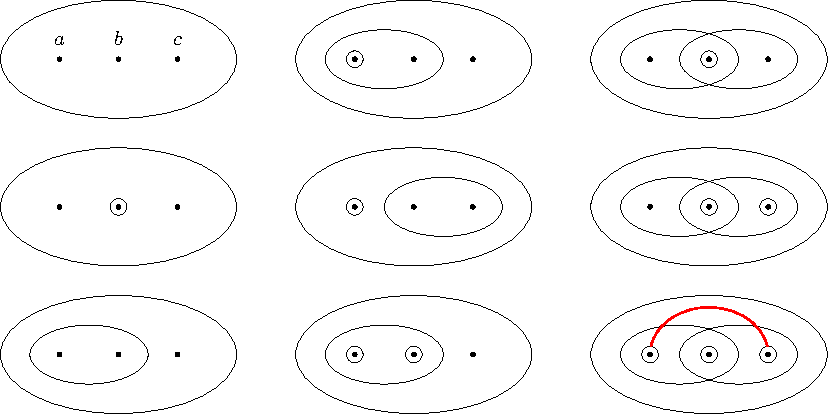
\includegraphics{fig/ch2-top.pdf}
    \caption{$a,b,c$的拓扑}\label{chtop:pic_top}
\end{figure}



\begin{definition}\label{chtop:eqn_neighbor}
    设$(X,\mathscr{T})$为拓扑空间,$\forall x\in N \subset X$,
    如果存在开集$U\in \mathscr{T}$使得$x\in U \subset N $,
    则称$N$为$x$的{\heiti 邻域}.如果$N$本身是开集,则称为{\heiti 开邻域}.
    \index[physwords]{邻域}
\end{definition}

\begin{definition}\label{chtop:def_Hausdorff}
    设拓扑空间$X$中有任意两个不同的点$x$和$y$,
    如果有不相交的($U \cap V = \varnothing$)邻域$U$和$V$分别包含它们,
    即$x\in U$和$y\in V$,则称$X$为{\bfseries \heiti Hausdorff空间}.
    \index[physwords]{Hausdorff空间} \index[persons]{Hausdorff}
\end{definition}





\begin{definition}\label{chtop:def_closedset}
    设$U$是拓扑空间$X$的子集,若$X-U$是开集,
    则称$U$为{\heiti 闭集}. \index[physwords]{闭集}
\end{definition}


\begin{definition}\label{chtop:def_cartensian}
    设有两个非空集合$A$和$B$,所有有序偶对$(a,b)$(其中$a\in A, b\in B$)的集合
    定义为{\heiti 笛卡尔积},简称为{\heiti 积},
    记为$A \times B = \{(a,b)| a\in A, b\in B \}$.\index[physwords]{笛卡尔积}
\end{definition}
需要注意$a$和$b$的顺序不能随意调换;
定义\ref{chtop:def_cartensian}可以拓展到有限个集合情形.
这里只给出了最简单“积”的概念,更详细描述见文献\parencite[\S 1, \S5, \S 15, \S19]{munkres-2000-topology}.



%\section{$\mathbb{R}^m$上的拓扑学}\label{chtop:sec_RmTP}

\section{度量空间}
\begin{definition}\label{chtop:def_metric}
    集合$X$的一个{\heiti 度量}是一个函数:$d:X\times X \to \mathbb{R}$;
    它使得以下性质成立:
    {\bfseries (1)} $\forall x,y \in X$,$d(x,y) \geqslant 0$;等号当且仅当$x=y$时成立.
    {\bfseries (2)} $\forall x,y \in X$,$d(x,y) =d(y,x)$.
    {\bfseries (3)} $\forall x,y,z \in X$,$d(x,y) +d(y,z) \geqslant d(x,z)$.
\end{definition}


定义\ref{chtop:def_metric}中的度量是拓扑学上的度量;
之后,我们还会在线性空间、黎曼流形上引入度量概念;它们各有异同.

\begin{definition}
    集合$X$连同给定的度量$d$称为{\heiti 度量空间},记为$(X,d)$.
\end{definition}


给定$X$一个度量$d$,实数$d(x,y)$通常称为$x$和$y$之间在$d$下的{\heiti 距离}.
对于$\varepsilon >0$,考虑所有与$x$的距离小于$\varepsilon$的点$y$的集合
\begin{equation}\label{chtop:eqn_eball}
    B_{d}(x,\varepsilon)\equiv \{y \ |\ d(x,y)<\varepsilon\} .
\end{equation}
$B_{d}(x,\varepsilon)$称为{\heiti 以$x$为中心的$\varepsilon$-球}.
在不引起混淆的前提下,可以记成$B(x,\varepsilon)$.

例如$\mathbb{R}^m$具有下列两个常用度量(请读者验证下两式符合度量定义):
\begin{subequations}\label{chtop:eqn_Rdbc}
    \begin{align}
        d_b(\boldsymbol{x}, \boldsymbol{y})=& \|\boldsymbol{x}-\boldsymbol{y}\|
        =\sqrt{(x^1-y^1)^2+\cdots +(x^m-y^m)^2}, \label{chtop:eqn_Rdb} \\
        d_c(\boldsymbol{x}, \boldsymbol{y})=& |\boldsymbol{x}-\boldsymbol{y}|
        =\max\{|x^1-y^1|,\cdots,|x^m-y^m| \}. \label{chtop:eqn_Rdc}
    \end{align}
\end{subequations}
分别称为 欧几里得 度量和确界度量;
欧几里得度量的几何意义是以$x$为中心的$\varepsilon$-球$B_{d}(x,\varepsilon)$;
确界度量的几何意义是以$\boldsymbol{x}$为中心以 $\varepsilon$ 为半边长的开立方体,
记为$C(\boldsymbol{x} , \varepsilon)$.
不难验证不等式$|\boldsymbol{x}| \leqslant\|\boldsymbol{x}\| \leqslant \sqrt{m}|\boldsymbol{x}|$成立,
它导致下列包含关系:
\begin{equation}\label{chtop:eqn_BCB}
    B(\boldsymbol{x} , \varepsilon) \subset C(\boldsymbol{x} , \varepsilon)
     \subset B(\boldsymbol{x} , \sqrt{m} \varepsilon) .
\end{equation}

需要强调的是拓扑空间定义并不需要度量,但由度量诱导的拓扑更加直观.
为了描述简单起见,我们尽量使用度量诱导出来的拓扑(比如$\mathbb{R}^m$中的拓扑),
这样更容易想象出几何图像.
%其实拓扑学中大部分内容都是从$(\mathbb{R}^m,d)$中抽象出来的.

\begin{theorem}\label{chtop:thm_RD}
    $B_{d}(x,\varepsilon)$会诱导出$(X,d)$上的一个拓扑.
\end{theorem}
\begin{proof}
    规定$X$子集族$\mathscr{T}_d \equiv \{
    U\ |\ U \text{是若干$\varepsilon$-球的并集}\}$.
    下面证明$(X, \mathscr{T}_d)$符合拓扑空间定义\ref{chtop:def_top}.
    证明过程就是验证$(X, \mathscr{T}_d)$符合定义\ref{chtop:def_top}中的三个公理.
    
    需要指出的是$B_{d}(x,\varepsilon)$中的$\varepsilon$可以等于$+\infty$或零;
    这样$\mathscr{T}_d$包含$\varnothing$和$X$本身;
    故$\mathscr{T}_d$满足定义\ref{chtop:def_top}中的第(1)条.
    
    很明显,任意个$\varepsilon$-球的并集仍在$\mathscr{T}_d$中;
    验证了\ref{chtop:def_top}中的第(2)条.
    
    为了证明第(3)条,我们需要先证明一个引理.
    设$B_{d}(x_1,\varepsilon_1)$、$B_{d}(x_2,\varepsilon_2)$是$(\mathbb{R}^m,d)$的
    两个$\varepsilon$-球,再假设它们的交集非空,
    即$\varnothing\neq U= B_{d}(x_1,\varepsilon_1)\cap B_{d}(x_2,\varepsilon_2)$.
    $\forall y \in U$,不难得到:$\varepsilon_i - d(y,x_i) >0 \, (i=1,2)$.
    记$\varepsilon_y= \min \{\varepsilon_1 - d(y,x_1),\ \varepsilon_2 - d(y,x_2)\}$,
    易证$B_{d}(y,\varepsilon_y)\subset U$;
    于是有$U = \bigcup_{y\in U} B_{d}(y,\varepsilon_y)$,
    也就是:{\kaishu $(X,d)$上任意两个$\varepsilon$-球的交集是
        若干$\varepsilon$-球的并集.}
    
    设$U,U'\in \mathscr{T}_d$,记$U= \bigcup_{\alpha} B_{d}(y_\alpha,\varepsilon_\alpha)$、
    $U'= \bigcup_{\beta} B_{d}(y'_\beta,\varepsilon'_\beta)$.那么
    \begin{align*}
        U \cap U' = \left( \bigcup_{\alpha} B_{d}(y_\alpha,\varepsilon_\alpha) \right)
        \cap \left( \bigcup_{\beta} B_{d}(y'_\beta,\varepsilon'_\beta) \right)
        = \bigcup_{\alpha,\beta }\left( B_{d}(y_\alpha,\varepsilon_\alpha)
        \cap B_{d}(y'_\beta,\varepsilon'_\beta) \right).
    \end{align*}
    根据刚刚证明的引理,对于任何$\alpha,\beta$,$B_{d}(y_\alpha,\varepsilon_\alpha)
    \cap B_{d}(y'_\beta,\varepsilon'_\beta) \in \mathscr{T}_d$;
    再由拓扑公理(2)可以得出$U\cap U'\in \mathscr{T}_d$.
    这便证明了$\mathscr{T}_d$满足第(3)条公理.
\end{proof}

定理\ref{chtop:thm_RD}中的$\mathscr{T}_d$称为由度量$d$诱导出来的{\heiti 度量拓扑}.
该定理自然适用于$(\mathbb{R}^m,d)$.


下面讨论$\mathbb{R}^m$上{\heiti 标准开集}的概念;
需要注意{\kaishu 标准开集}的概念是人为规定的.
实数轴$\mathbb{R}$中的开区间$(a,b)$是{\kaishu 标准开集};
闭区间$[a,b]$和半开半闭区间$[a,b)$、$(a,b]$和单点集都不是标准开集.推而广之,
以$x$为中心的$\varepsilon$-球\eqref{chtop:eqn_eball}是$\mathbb{R}^m$中的{\kaishu 标准开集}.
很明显,开球$B_{d}(x,\varepsilon)$是定义\ref{chtop:eqn_neighbor}中所描述的{\kaishu 开邻域}中的一种.

$\mathbb{R}^m$上一般开集定义(包括各种非标准开集)可参阅\parencite[\S 12,\S 13]{munkres-2000-topology}.
由于我们基本不会涉及这些非标准开集,故之后的行文中将省略“标准”二字.

因$(a,b)$是$\mathbb{R}$中的开集,由定义\ref{chtop:def_closedset}可知
$(-\infty, a]$、$[b,+\infty)$以及单点集都是闭集.
$[a,b]$称为$(a,b)$的{\kaishu 闭包}.
而半开半闭集合既不是开集也不是闭集,不是$(\mathbb{R},\mathscr{T}_d)$中的元素.

包含关系\eqref{chtop:eqn_BCB}蕴涵着下列定理:
\begin{theorem}\label{chtop:thm_bcb}
    若 $X$ 是 $\mathbb{R}^m$ 的一个子空间,那么无论是用 $X$上的欧几里得度量
    还是按确界度量,$X$ 的开集族是相同的; 对于 $X$ 的闭集族也同样成立.    
\end{theorem}

定理\ref{chtop:thm_bcb}表明:对于大多数拓扑问题来说,$\mathbb{R}^m$上的这两个度量是等价的.




\begin{definition}\label{chtop:def_induced-top}
    设$A$是拓扑空间$(X,\mathscr{T})$的一个非空子集,构建如下子集
    族$\mathscr{T} _A \equiv \{U\cap A \mid U\in \mathscr{T}\}$.
    称$\mathscr{T}_A$是$A$上的{\heiti 子空间拓扑}或从$(X,\mathscr{T})$得到的{\heiti 诱导拓扑}.
    \index[physwords]{诱导拓扑}
\end{definition}

我们对诱导拓扑做一下解释.现有二维平面$\mathbb{R}^2$和一维实直线$\mathbb{R}$,
二维平面采用标准拓扑,即开圆盘$B(x,\varepsilon)$之并.
$\mathbb{R}$显然是$\mathbb{R}^2$的非空子集;
通过诱导拓扑定义\ref{chtop:def_induced-top}可以看到:
实直线与开圆盘$B(x,\varepsilon)$交集就是开区间,因此诱导拓扑就是实直线上的标准拓扑.
还有一点需要注意,这个诱导拓扑用二维平面上开集(开圆盘)来衡量并不是开集,
因为没有宽度的实直线不可能装下开圆盘.


\begin{definition}\label{chtop:def_bases}
    设有拓扑空间$(X,\mathscr{T})$,以及$X$上的一组开集族$\mathscr{B}$.
    若$\forall A \in \mathscr{T}$,它都可以表示成$\mathscr{B}$中若干元素的并集,
    则称$\mathscr{B}$是拓扑空间$(X,\mathscr{T})$的{\heiti 拓扑基 }.%简称{\heiti 基}.
\end{definition}

不难验证开球$B_d(x,\varepsilon)$是度量空间$(X,d)$的拓扑基.
由定义可见拓扑基本身就是$X$的一个拓扑,其它开集都可以由基中元素表出;
这类似于三维欧氏空间中的三个基矢量,其它矢量都可以由三个基矢线性表出.

\begin{definition}
    一个拥有无限多个元素的集合$A$,如果其中元素和正整数集合有双射关系,
    则称$A$是{\heiti 可数的}(countable).
\end{definition}
有限集合自然可以和正整数集合的某个子集建立双射关系,故必然可数.



\section{连续性}

\begin{definition}\label{chtop:def_continuity}
    设$X$和$Y$是两个拓扑空间,存在映射$f:X\to Y$,如果对于$Y$中的每个
    开子集$V$,$f^{-1}(V)$是$X$中的一个开子集,则称映射$f$为{\heiti 连续的}.
\end{definition}

我们解释一下定义\ref{chtop:def_continuity}中的集合
\begin{equation}
    f^{-1}(V)=\{x \mid  f(x) \in V\},
\end{equation}
它是$X$中所有使得$f(x)\in V$的点$x$的集合;如果$V$与$f$的像集无交,则$f^{-1}(V)=\varnothing$.
特别需要注意$f^{-1}$不是逆映射,是逆像的集合.

%连续性可以用包含度量的方式表述,
设$X$、$Y$中分别有度量$d_X$、$d_Y$,
函数 $f$ 在 $x_0$ 点连续;那么,对任意$\varepsilon>0$,
都存在一个相应的 $\delta>0$ 使得当 $d_X(x, x_0)<\delta$ 时,
$d_Y\bigl(f(x), f(x_0)\bigr)<\varepsilon $成立.
这就是连续性的经典 $\varepsilon-\delta$ 表述法.
%同时读者应能看出定义\ref{chtop:def_continuity}是$\varepsilon-\delta$ 表述法在拓扑学中的抽象表述.

注意到对给定的 $x_0 \in X$,也可能恰巧对每个 $\delta>0$,$ x_0$ 的 $\delta$ 邻域只包含 $x_0$ 点.
在这种情况下, 将 $x_0$ 称为 $X$ 的孤立点, 任何函数 $f: X \rightarrow Y$ 在孤立点自动是连续的!



\begin{example}\label{chtop:exm_txyr}
    连续性和$X$、$Y$拓扑的关系.
\end{example}
比如$X$选为$\mathbb{R}$,拓扑是{\kaishu 标准拓扑}.
$Y$也选为$\mathbb{R}$,但将拓扑选为所谓的{\kaishu 下限拓扑},即$\mathbb{R}$中的
半开半闭区间$[a,b)$是开集,同时将其记为$\mathbb{R}_\ell$.写到这里需要对拓扑再做些
说明,拓扑的规定是十分任意的,也是人为的,只要符合拓扑三公理即可,下限拓扑完全符合
拓扑三公理,请读者自行验证或参考\parencite[\S 13]{munkres-2000-topology}中的$\mathbb{R}_K$拓扑定义.
现在,我们选恒等映射
\begin{equation}
    \imath : \mathbb{R} \to \mathbb{R}_\ell,\quad
    \text{即对于任意一个实数}x,\  \imath(x) =x .
\end{equation}
但是映射$\imath${\kaishu 不是}一个连续函数.因为$\mathbb{R}_\ell$中的开集$[a,b)$的
原像还是$[a,b)$,它不是$\mathbb{R}$(标准拓扑)中的开集. \qed

\begin{definition}\label{chtop:def_homeomorphism}
    设$X$和$Y$是两个拓扑空间,如果存在双射$f:X\to Y$,并且$f$和$f^{-1}$是
    连续的,则称映射$f$为{\heiti 同胚}. 此处指整体同胚.  \index[physwords]{同胚}
\end{definition}

正是因为有例\ref{chtop:exm_txyr}这种情形,定义\ref{chtop:def_homeomorphism}中
必须同时满足$f$、$f^{-1}$连续.
在同胚映射下不变的属性称为{\heiti 拓扑性质}(topological property);
比如紧致就是拓扑性质的例子.


\begin{definition}\label{chtop:def_topological-manifold}
    设$X$为具有可数拓扑基的Hausdorff空间,若它的每一点$x$都有一个开邻域$U$同胚于$\mathbb{R}^m$中的
    一个标准开子集,则称$X$为$m$维{\heiti 拓扑流形}.\index[physwords]{拓扑流形}
\end{definition}

定义\ref{chtop:def_topological-manifold}中{\kaishu 维数}是一个很复杂的问题,
请参阅\parencite[\S 50]{munkres-2000-topology}.
此处我们简单地认为流形$X$只有一个维数,就是$m$;不考虑其它复杂情形.
代数拓扑学中有一个基本定理:  %(可参见\parencite[p. 126]{hatcher-2002-at}定理2.26)
设有两个非空标准开集$U\subset \mathbb{R}^m$、$V\subset \mathbb{R}^n$,
如果$U$、$V$相互同胚,那么它们的维数相等,即$m=n$.


微积分中有许多定理可以推广到度量空间(或一般拓扑空间)中,我们不加证明
(可参考\parencite{munkres-2000-topology}定理18.2、18.4、21.5)的叙述两个.
下面定理中$X$、$Y$均是度量空间.

\begin{theorem}
    {\bfseries (1)} 若$f:X\to Y$将整个$X$映射为$Y$中一个点$y_0$,则$f$是连续的;即常值映射是连续的.
    {\bfseries (2)} 令 $x_0 \in A$,这里 $A$ 是 $X$ 的一个子空间.
    如果 $f: X \rightarrow Y$ 在 $x_0$点是连续的,那么限制函数 $\left.f\right|_A: A \rightarrow Y$
    在 $x_0$ 点也是连续的.
    {\bfseries (3)} 令 $f: X \rightarrow Y$,$g: Y \rightarrow Z$.
    若 $f$ 在 $x_0$ 点连续且 $g$ 在 $y_0=f\left(x_0\right)$ 点连续,
    那么 $g \circ f: X \rightarrow Z$ 在 $x_0$ 点连续.
\end{theorem}


\begin{theorem}
    {\bfseries (1)} 令$f: X \rightarrow \mathbb{R}^m$ 具有下列形式:
    $    f(x)=\bigl(f_1(x), \cdots, f_m(x)\bigr)     $    .
    那么当且仅当每个函数$f_{i}: X \rightarrow \mathbb{R}$ 在 $x_0$ 点连续时,
    $f$ 在 $x_0$ 点连续;各$f_i$称为 $f$的分量函数.    
    {\bfseries (2)} 令 $f, g: X \rightarrow \mathbb{R}$ 在 $x_0$ 点连续;
    那么 $f+g, f-g$ 及 $f \cdot g$ 均在 $x_0$ 点连续,并且当 $g(x_0) \neq 0$ 时 $f / g$ 在 $x_0$ 点连续.
    {\bfseries (3)} 投影函数$\pi_i(\boldsymbol{x})=x_i$($x_i$是$\boldsymbol{x}$第$i$分量)是连续的.
\end{theorem}










\section{拓扑空间的数个重要属性}
我们不加证明(可参考本章末文献)地列举一些拓扑空间的重要属性.


%\section{紧致性}
\begin{definition}\label{chtop:def_covering}
    给定拓扑空间$(X,\mathscr{T})$,设$\{U_\alpha\}, \alpha\in \mathbb{I}$是$X$的一个
    子集族,如果$\{U_\alpha\}$的成员之并等于$X$,则称$\{U_\alpha\}$为$X$的{\heiti 覆盖}.
    若$\{U_\alpha\}$每个成员都是开子集,则称为{\heiti 开覆盖}.
    \index[physwords]{开覆盖}
\end{definition}

\begin{definition}\label{chtop:def_compact}
    若拓扑空间$X$任意开覆盖$\{U_\alpha\}$都
    有\uwave{有限子族}能覆盖$X$,则称$X$为{\heiti 紧致的}.
    \index[physwords]{紧致}
\end{definition}



\begin{proposition}
    紧致空间的每一个闭子集都是紧致的.
\end{proposition}


\begin{proposition}
    Hausdorff空间的每一个紧致子空间都是闭的.
\end{proposition}


\begin{proposition}
    紧致空间在连续映射下的像集也是紧致的.
\end{proposition}

\begin{proposition}
    有限个紧致空间的笛卡尔积也是紧致的.
\end{proposition}


\begin{proposition}
    $\mathbb{R}^m$中子集$A$是紧致的充要条件是$A$是闭集且在度量\eqref{chtop:eqn_Rdbc}下有界.
\end{proposition}

\begin{definition}
    空间$X$在{\heiti\bfseries 点$x$是局部紧致的}是指:若存在$X$的一个紧致子空间$C$包含着$x$的一个邻域.
    若$X$在每一点都是局部紧致的,则称$X$是{\heiti 局部紧致的}.
\end{definition}


实直线并不是紧致空间,然而它是局部紧致的;$\forall x\in \mathbb{R}$,存在一个包含它的开邻域$x\in (a,b)$,
而这个开邻域必然包含在紧致子集$[a,b]$之中.推而广之,$\mathbb{R}^m$是局部紧致的,但整体上并非紧致.

\begin{theorem}
    Hausdorff空间$X$在$x$处局部紧致的充要条件是:对于$x$的任意邻域$U$,存在一个邻域$V$,
    使得$\bar{V}$紧致并且$\bar{V}\subset U$.
\end{theorem}

\begin{proposition}
    设$X$是局部紧致的Hausdorff空间,$A$是$X$的子集.
    若$A$是$X$的闭子集或开子集,则$A$是局部紧致的.
\end{proposition}

%\section{title}

\begin{proposition}
    $(\mathbb{R}^m, d_b)$是具有可数拓扑基的Hausdorff空间.
\end{proposition}

\begin{proposition}
    Hausdorff空间的拓扑子空间仍是Hausdorff空间.
\end{proposition}


\begin{proposition}\label{chtop:thm_hcb}
    有可数拓扑基的Hausdorff空间的拓扑子空间也有可数拓扑基.
\end{proposition}

\begin{proposition}
    设$\{U_i\}$、$\{V_j\}$分别是拓扑空间$X$、$Y$的拓扑基,
    那么$\{U_i\times V_j\}$(笛卡尔积)是$X\times Y$(笛卡尔积)的拓扑基.
\end{proposition}

\begin{proposition}\label{chtop:thm_cph}
    Hausdorff空间的笛卡尔积空间仍是Hausdorff空间.
\end{proposition}

\begin{proposition}
    有可数拓扑基的空间的笛卡尔积空间仍有可数拓扑基.
\end{proposition}




%\section{连通性}
\begin{definition}\label{chtop:def_connection}
    若拓扑空间$X$没有既开又闭的子集(除$X,\varnothing$外),
    则称$X${\heiti 连通}.\index[physwords]{连通}
\end{definition}

\begin{proposition}
    连通空间在连续映射下的像集也是连通的.
\end{proposition}

\begin{proposition}
    有限个连通空间的笛卡尔积也是连通的.
\end{proposition}


%\section{完备性}
\begin{definition}\label{chtop:def_complete-metric}
    给定度量空间$(X,d)$,
    $X$中的序列$\{x_n\}$称为Cauchy序列是指:$\forall \epsilon >0 $,存在正整数$N$使
    得$d(x_n,x_m)<\epsilon,\ \forall n,m>N$成立.如果$X$中的每个Cauchy序列
    都是收敛的(极限点属于$X$),则称$X$是{\heiti 度量完备}的,简称{\heiti 完备}.
    \index[physwords]{完备} \index[physwords]{完备!度量完备}
\end{definition}

\begin{proposition}
    对于度量\eqref{chtop:eqn_Rdbc}而言,欧氏空间$\mathbb{R}^m$是完备的.
\end{proposition}

\begin{example}
    在度量\eqref{chtop:eqn_Rdc}意义下,有$\mathbb{R}$中开区间$(-1,1)$的
    序列$\{x_n=1-1/n\}$,这是一个Cauchy序列.此序列的极限点是$1$,
    然而$1 \notin (-1,1)$,故它不完备.
    
    已知$(-1,1)$同胚于实直线$\mathbb{R}$,而$\mathbb{R}$是完备的;
    故{\kaishu 完备不是拓扑属性}.\qed
\end{example}

%\section{代数拓扑初步}\label{chtop:sec_at}

%将代数拓扑单列一节的目的是在于强调它不同于点集拓扑,从定义伊始就不同.
代数拓扑完全超出了本书的范畴,请参阅\parencite{munkres-2000-topology};
我们只给出一个定义.

\begin{definition}\label{chtop:def_covering-map}
    设$E,B$均是连通的Hausdorff空间,$p:E\to B$是连续映射.
    若$\forall b\in B$有开邻域$U$使$p^{-1}(U)$为$E$的一族两两不相交的
    开集$\{V_\alpha\}$的并集,并且$p$把每个$V_\alpha$同胚地映射成$U$,
    则称$p$为{\heiti 覆叠映射};
    $(E,p)$为$B$上的{\heiti 覆叠空间},$B$为$E$的{\heiti 底空间};
    称$U$为$b$的{\heiti 基本邻域};
    每个$V_\alpha$叫作$p^{-1}(U)$的{\heiti 分支};
    $\forall b\in B$,$p^{-1}(b)$称为$b$上的{\heiti 纤维}.
    \index[physwords]{覆叠映射} \index[physwords]{覆叠空间}
\end{definition}

%定义\ref{chtop:def_covering}中的覆盖和定义\ref{chtop:def_covering-map}中的覆叠的英文
%都是“cover”.定义\ref{chtop:def_covering}是点集拓扑中的概念;
%定义\ref{chtop:def_covering-map}是代数拓扑中的概念,“覆叠”也被翻译成“复叠”、“覆盖”.
%如果把定义\ref{chtop:def_covering-map}中的“Hausdorff空间”换成“微分流形”(见\ref{chdm:def_Dmanifold}),
%再把“同胚”换成“微分同胚”(见\ref{chdm:def_Diff-Homeomorphism}),那么上述
%覆叠映射便是微分流形间的覆叠映射.







\section*{小结}
本章初步介绍了点集拓扑的知识,是不完备的;
详尽内容可参考文献\parencite{munkres-2000-topology}.




\printbibliography[heading=subbibliography, title=第\ref{chtop}章参考文献]
\endinput
